\documentclass{article}
\usepackage{tikz}
\usepackage{wrapfig} 
\usepackage{amsmath} 
\usepackage[a4paper]{geometry}
\usepackage{fancyhdr}
\pagestyle{fancy}
\lhead{Vektoren}
\rhead{März 2025}
\begin{document}
 
\newcommand{\norm}[1]{\left| {#1} \right|}  
\newcommand{\vect}[1]{\overrightarrow{#1}} 
 
\section{Vektoren}
Ein Vektor beschreibt die Verschiebung, sei diese zweidimensionalen Koordinatensystem oder einem dreidimensionalen Raum. Somit beschreiben sie sowohl eine Länge als auch eine Richtung. In Skizzen werden sie ale Pfeile dargestellt. Vektoren werden aufgeschrieben, indem die Koordinaten, welche $x$, $y$ und $z$ bzw. $x_1$, $x_2$ und $x_3$ genannt werden, untereinander aufgelistet werden, in der Form 
\[
 \vect{x} = \begin{pmatrix} x \\ y \end{pmatrix}
 \quad \text{oder} \quad
 \begin{pmatrix} x_1 \\ x_2 \end{pmatrix}
\]
bzw. 
\[
 \vect{x} = \begin{pmatrix} x \\ y \\ z \end{pmatrix}
 \quad \text{oder} \quad
 \begin{pmatrix} x_1 \\ x_2 \\ x_3 \end{pmatrix}
\]
  
\section{Spezielle Vektoren}
Es gibt verschiedene spezielle Arten von Vektoren, mit verschiedenen Eigenschaften.
\begin{description}
 \item[Nullvektor] Ein Nullvektor ist ein Vektor, bestehend aus nur Nullen.
\[
 \vect{0} = \begin{pmatrix} 0 \\ 0 \end{pmatrix}
\]
 
 \item[Gegenvektoren] Das Gegenteil eines Vektors $\vect{v}$, welcher die gegenteiligen Koordinaten hat, ist der Gegenvektor, $-\vect{v}$. \end{description} 
 
\noindent
\begin{minipage}{\dimexpr\textwidth-5cm}  % Adjust width as needed
 \begin{description}
  \item[Verbindungsvektoren] Ein Verbindungsvektor beschreibt einen Vektor, welcher zwei Punkte verbindet. Der Wert eines Verbindungsvektors ist die differenz zwischen den zwei Punkten; wie weit der erste Punkt verschoben werden müsste, um den zweiten zu erreichen. So gilt für den Verbindungsvektor der Punkt $\mathrm{P}$ und $\mathrm{Q}$
\[
 \vect{\mathrm{PQ}} =
 \begin{pmatrix}
  \mathrm{q}_1 - \mathrm{p}_1 \\
  \mathrm{q}_2 - \mathrm{p}_2
 \end{pmatrix}
\] 
 \end{description} 
\end{minipage}%
\hfill
\begin{minipage}{5cm}  % Adjust width as needed
  \centering
  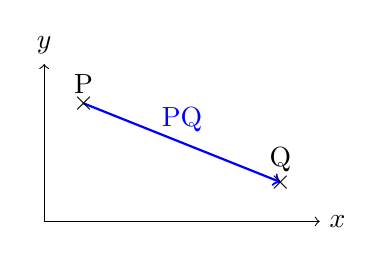
\begin{tikzpicture}
  \draw[->] (0,0) -- (3.5,0) node[right] {$x$};
  \draw[->] (0,0) -- (0,2) node[above] {$y$};
 
  \draw[->, thick, blue] (0.5,1.5) -- (3,0.5) node[midway, above] {$\vect{\mathrm{PQ}}$};  
 
  \draw (0.5,1.5) node {$\times$} node[above] {P}; 
  \draw (3,0.5) node {$\times$} node[above] {Q}; 
  \end{tikzpicture}
\end{minipage} 
 
\begin{description} 
 \item[Ortsvektoren] Der Ortsvektor eines Punktes ist der Verbindungsvektor, welcher vom Koordinatenursprung $\mathrm{O}$ zu diesem Punkt geht. So ist der Ortsvektor vom Punkt $\mathrm{P}$ der Vektor $\vect{\mathrm{OP}}$. Weil $\mathrm{O}$ durch einen Nullvektor repräsentiert werden kann, sind die Koordinaten des Ortsvektors $\vect{\mathrm{OP}}$ dieselben wie die vom Punkt $\mathrm{P}$
\end{description} 
 
\subsection{Addition} 
Vektoren können, genau wie normale Zahlen auch, miteinander addiert und subtrahiert werden. Die Summe zweier Vektoren kann als beide einzelnen Vektoren, wobei der Anfang des einen and das Ende des anderen gelegt wurde, angesehen werden. \newline 
\begin{wrapfigure}[6]{l}{5cm}
  \centering
  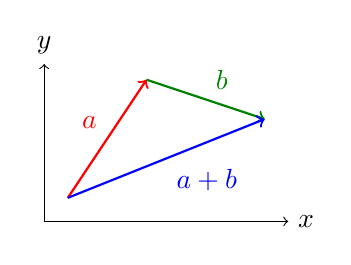
\begin{tikzpicture}
    \draw[->] (0,0) -- (3.1,0) node[right] {$x$};
    \draw[->] (0,0) -- (0,2) node[above] {$y$};
 
    \draw[->, thick, red] (0.3,0.3) -- ++(1,1.5) node[midway, above left] {$\vect{a}$};
    \draw[->, thick, green!50!black] (1.3,1.8) -- ++(1.5,-0.5) node[midway, above right] {$\vect{b}$};
    \draw[->, thick, blue] (0.3,0.3) -- ++(2.5,1) node[midway, below right] {$\vect{a} + \vect{b}$};  
  \end{tikzpicture}
\end{wrapfigure}
Algebraisch wird dabei die jeweilige Rechenart nur auf die einzelnen Koordinatenpaare angewand, heißt 
\[ 
 \begin{pmatrix} a_1 \\ a_2 \end{pmatrix} +
 \begin{pmatrix} b_1 \\ b_2 \end{pmatrix} =
 \begin{pmatrix} a_1 + b_1 \\ a_2 + b_2 \end{pmatrix} 
\]
Gleiches gilt für subtraktion, mit $\vect{a} - \vect{b} = \vect{a} + (-\vect{b})$.
 
\subsection{Multiplikation}
\begin{wrapfigure}{r}{5cm}
  \centering
  \raisebox{-2cm}[0pt]{
  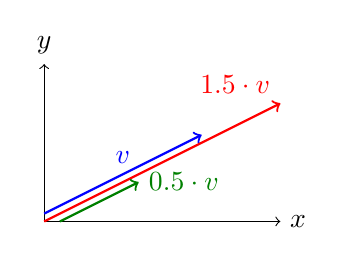
\begin{tikzpicture}
    \draw[->] (0,0) -- (3,0) node[right] {$x$};
    \draw[->] (0,0) -- (0,2) node[above] {$y$};
 
    \draw[->, thick, blue] (0,0.1) -- ++(2,1) node[midway, above] {$\vect{v}$};
 
    \draw[->, thick, red] (0,0) -- (3,1.5) node[above left] {$1.5 \cdot \vect{v}$};
 
    \draw[->, thick, green!50!black] (0.2,0) -- ++(1,0.5) node[right] {$0.5 \cdot \vect{v}$};
  \end{tikzpicture}} 
\end{wrapfigure}
Vektoren können mit Zahlen multipliziert werden, wodurch die Länge dem Faktor nach verlängert oder verkürzt wird. Algebraisch wird dabei die Multiplikation auf die einzelnen Koordinatenpaare angewand, heißt
\[ 
 r \cdot
 \begin{pmatrix} x_1 \\ x_2 \end{pmatrix} =
 \begin{pmatrix} r \cdot x_1 \\ r \cdot x_2 \end{pmatrix} 
\]
 
\subsection{Beträge}
\begin{wrapfigure}{l}{5cm}
  \centering
  \raisebox{-1.7cm}[0pt]{
  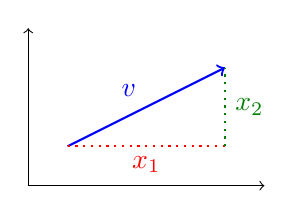
\begin{tikzpicture}
    \draw[->] (0,0) -- (3,0);% node[right] {$x_1$};
    \draw[->] (0,0) -- (0,2);% node[above] {$x_2$};
 
    \draw[->, thick, blue] (0.5,0.5) -- ++(2,1) node[midway, above left] {$\norm{\vect{v}}$};
 
    \draw[dotted, thick, red] (0.5,0.5) -- ++(2,0) node[midway, below] {$x_1$};
 
    \draw[dotted, thick, green!50!black] (2.5,0.5) -- ++(0,1) node[midway, right] {$x_2$};
  \end{tikzpicture}}
\end{wrapfigure}
Der Betrag eines Vektors spiegelt die Länge wieder. Diese wird mit einer Formel, hergeleitet vom Satz des Pythagoras, berechnet, wobei der Vektorenpfeil als Hypothenuse eines Dreiecks mit den Vektorenkoordinaten als Katheten gesehen wird. Somit gilt
\[
 \norm{\vect{v}} =
 \sqrt{{x_1}^2 + {x_2}^2}
\]
 
\subsection{Kollinearität} 
Zwei Vektoren sind kollinear, wenn sie in die gleiche Richtung zeigen, also einer nur ein Vielfache des anderen ist. Kollinearität zwischen $\vect{a}$ und $\vect{b}$ ist vorhanden, wenn es ein $r$ gibt, so dass 
\[ 
 r \cdot \vect{a} = \vect{b}
\]
 
\subsection{Linearkombinationen} 
Ein Vektor, welcher als Summe von den Vielfachen zweier Vektoren dargestellt werden kann, ist ein Linearkombination dieser. $\vect{c}$ ist eine Linearkombination von $\vect{a}$ und $\vect{b}$, wenn
\[
 \vect{c} = r \cdot \vect{a} + s \cdot \vect{b} 
\]
erfüllt sein kann. Dies kann überprüft werden, indem die obige Gleichung als lineares Gleichungssystem aufgeschrieben wird  und nach $r$ und $s$ aufgelöst wird.
 
\end{document}
 
 
 
 
 
 
 
 
 
 
 
 
 
 
 
 
 
